
%%%%%%%%%%%%%%%%%%%%%%%%%%%%%%%%%%%%%%%%%%%%%%%%%%%%%%%%%%%%%%%%%%%%%%%%%%%%%%%%%%%%%%%
%%%%%%%%%%%%%%%%%%%%%%%%%%%%%%%%%%%%%%%%%%%%%%%%%%%%%%%%%%%%%%%%%%%%%%%%%%%%%%%%%%%%%%%
% 
% This top part of the document is called the 'preamble'.  Modify it with caution!
%
% The real document starts below where it says 'The main document starts here'.

\documentclass[12pt]{article}

\usepackage{amssymb,amsmath,amsthm}
\usepackage[top=1in, bottom=1in, left=1.25in, right=1.25in]{geometry}
\usepackage{fancyhdr}
\usepackage{enumerate}
\usepackage{listings}
\usepackage{graphicx}
\usepackage{float}
\usepackage{multicol}
% Comment the following line to use TeX's default font of Computer Modern.
\usepackage{times,txfonts}
\usepackage{mwe}
\usepackage{caption}
\usepackage{subcaption}





\makeatletter
\renewcommand*\env@matrix[1][*\c@MaxMatrixCols c]{%
  \hskip -\arraycolsep
  \let\@ifnextchar\new@ifnextchar
  \array{#1}}
\makeatother

\newtheoremstyle{homework}% name of the style to be used
  {18pt}% measure of space to leave above the theorem. E.g.: 3pt
  {12pt}% measure of space to leave below the theorem. E.g.: 3pt
  {}% name of font to use in the body of the theorem
  {}% measure of space to indent
  {\bfseries}% name of head font
  {:}% punctuation between head and body
  {2ex}% space after theorem head; " " = normal interword space
  {}% Manually specify head
\theoremstyle{homework} 

% Set up an Exercise environment and a Solution label.
\newtheorem*{exercisecore}{Exercise \@currentlabel}
\newenvironment{exercise}[1]
{\def\@currentlabel{#1}\exercisecore}
{\endexercisecore}

\newcommand{\localhead}[1]{\par\smallskip\noindent\textbf{#1}\nobreak\\}%
\newcommand\solution{\localhead{Solution:}}

%%%%%%%%%%%%%%%%%%%%%%%%%%%%%%%%%%%%%%%%%%%%%%%%%%%%%%%%%%%%%%%%%%%%%%%%
%
% Stuff for getting the name/document date/title across the header
\makeatletter
\RequirePackage{fancyhdr}
\pagestyle{fancy}
\fancyfoot[C]{\ifnum \value{page} > 1\relax\thepage\fi}
\fancyhead[L]{\ifx\@doclabel\@empty\else\@doclabel\fi}
\fancyhead[C]{\ifx\@docdate\@empty\else\@docdate\fi}
\fancyhead[R]{\ifx\@docauthor\@empty\else\@docauthor\fi}
\headheight 15pt

\def\doclabel#1{\gdef\@doclabel{#1}}
\doclabel{Use {\tt\textbackslash doclabel\{MY LABEL\}}.}
\def\docdate#1{\gdef\@docdate{#1}}
\docdate{Use {\tt\textbackslash docdate\{MY DATE\}}.}
\def\docauthor#1{\gdef\@docauthor{#1}}
\docauthor{Use {\tt\textbackslash docauthor\{MY NAME\}}.}
\makeatother

% Shortcuts for blackboard bold number sets (reals, integers, etc.)
\newcommand{\Reals}{\ensuremath{\mathbb R}}
\newcommand{\Nats}{\ensuremath{\mathbb N}}
\newcommand{\Ints}{\ensuremath{\mathbb Z}}
\newcommand{\Rats}{\ensuremath{\mathbb Q}}
\newcommand{\Cplx}{\ensuremath{\mathbb C}}
%% Some equivalents that some people may prefer.
\let\RR\Reals
\let\NN\Nats
\let\II\Ints
\let\CC\Cplx
%%%%%%%%%%%%%%%%%%%%%%%%%%%%%%%%%%%%%%%%%%%%%%%%%%%%%%%%%%%%%%%%%%%%%%%%%%%%%%%%%%%%%%%
%%%%%%%%%%%%%%%%%%%%%%%%%%%%%%%%%%%%%%%%%%%%%%%%%%%%%%%%%%%%%%%%%%%%%%%%%%%%%%%%%%%%%%%
% 
% The main document start here.




%  \textbf{Code:}
%  \begin{center}
%  \lstinputlisting[basicstyle = \footnotesize]{}
%  \end{center}
%  
%  \begin{footnotesize}
%  \begin{verbatim}
%    
%  \end{verbatim}
%  \end{footnotesize}
%  
%  
%  \begin{figure}[H]
%    \begin{center}
%      \caption{}
%    \includegraphics[width = \textwidth]{}
%    \end{center}
%  \end{figure}





% The following commands set up the material that appears in the header.
\doclabel{Stat 605: Homework 6}
\docauthor{Stefano Fochesatto}
\docdate{\today}

\begin{document}

\begin{exercise}{1} Load the data into memory, data(wolfcamp); add a border to 
  the data set, plot it, discuss briefly. What are these data?\\
  \solution Loading the data and computing the border with my get.borders() 
  function we get the following plot of the data, 
  \begin{figure}[H]
    \begin{center}
      \caption{Plot of Wolfcamp data with border.}
    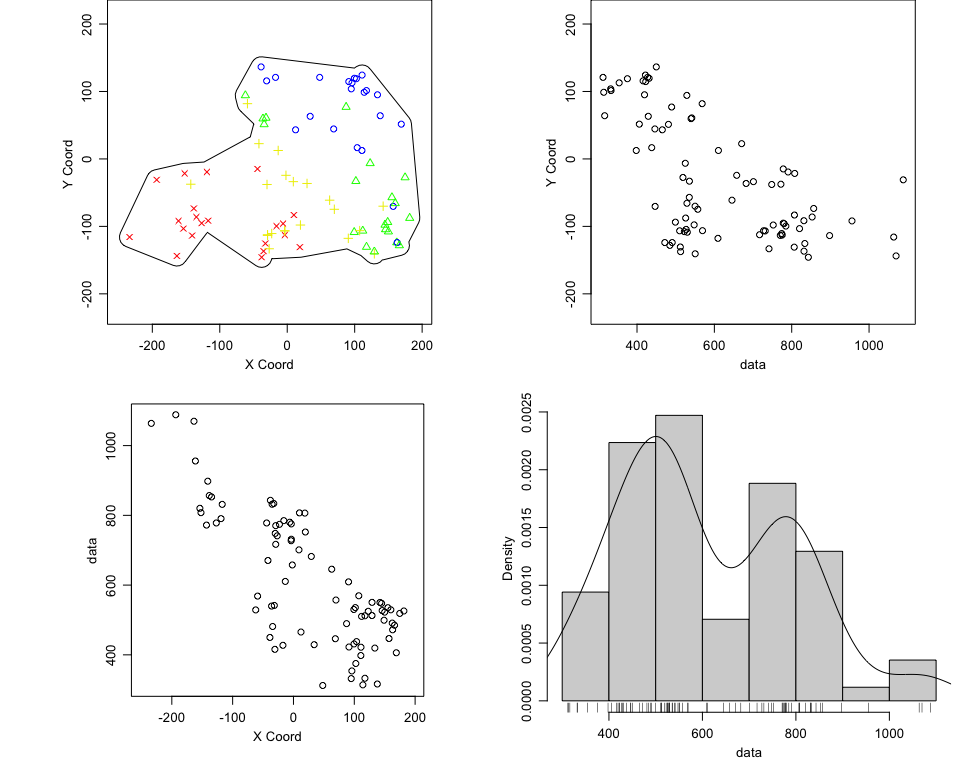
\includegraphics[width = \textwidth]{Rplot.png}
    \end{center}
  \end{figure}
    \textbf{Code:}
    \begin{center}
    \lstinputlisting[basicstyle = \footnotesize]{r1.txt}
    \end{center}
      From the description provided by the '? wolfcamp' command we find that the data are 
    Piezometric head measurements at various locations in the Wolfcamp aquifer located in Texas. 
    This data is a measure of pressure in an aquifer computed from the height of water in a tube.\\

    Recall that this same dataset was discussed in question question \#4 of homework \#2. In that exercise
    we concluded that there is a trend of increasing pressure as we move in the south west direction. We stated that the 
    partial dependence plots corroborated that assertion. We also found the data to be slightly right skewed, and log transforming it 
    produced a more centered, albeit still bimodal density histogram (We won't be using this transformation). 
    
    \begin{figure}[H]
      \begin{center}
        \caption{Plot of log transformed Wolfcamp data with border.}
      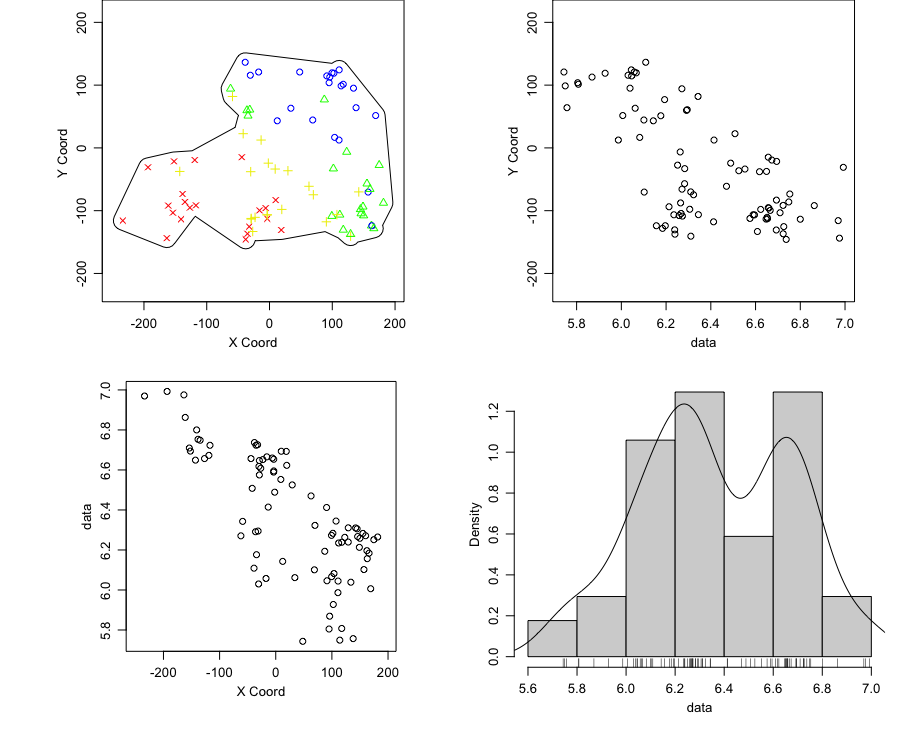
\includegraphics[width = \textwidth]{Rplot01.png}
      \end{center}
    \end{figure}
      \textbf{Code:}
      \begin{center}
      \lstinputlisting[basicstyle = \footnotesize]{r2.txt}
      \end{center}
\end{exercise}
\vspace{1in}






\begin{exercise}{2} Act as a frequentist; fit a spatial model to these data, and obtain a smoothed map. Did you include 
  a trend term or terms? Did you need to log-transform the data? Explain your reasoning. It might be helpful to show result from 
  fitting one or two multiple linear regression models.\\
  Be sure to discuss how you selected a type of semivariogram and how you estimated it's parameters. Be sure to state your final fitted model. 
  Discuss briefly. \\
  \solution To elaborate on the discussion on whether or not we should transform the data, I decided to perform a box-cox power analysis to see if we might find
  a worthwhile transformation. In doing so I found that we might want to consider the root transform, as well as the log transform. A Shapiro-Wilks test of normality on 
  all three candidate transforms concludes that they are sufficiently normal and looking at the qq norm plot, I don't 
  see a worthwhile difference between the transformations, so leaving the data alone seems to be the most parsimonious and interpretable option. \\
  \textbf{Code:}
  \begin{center}
  \lstinputlisting[basicstyle = \footnotesize]{r3.txt}
  \end{center}
  \begin{figure}[H]
    \begin{center}
      \caption{QQ normPlot of Wolfcamp data.}
    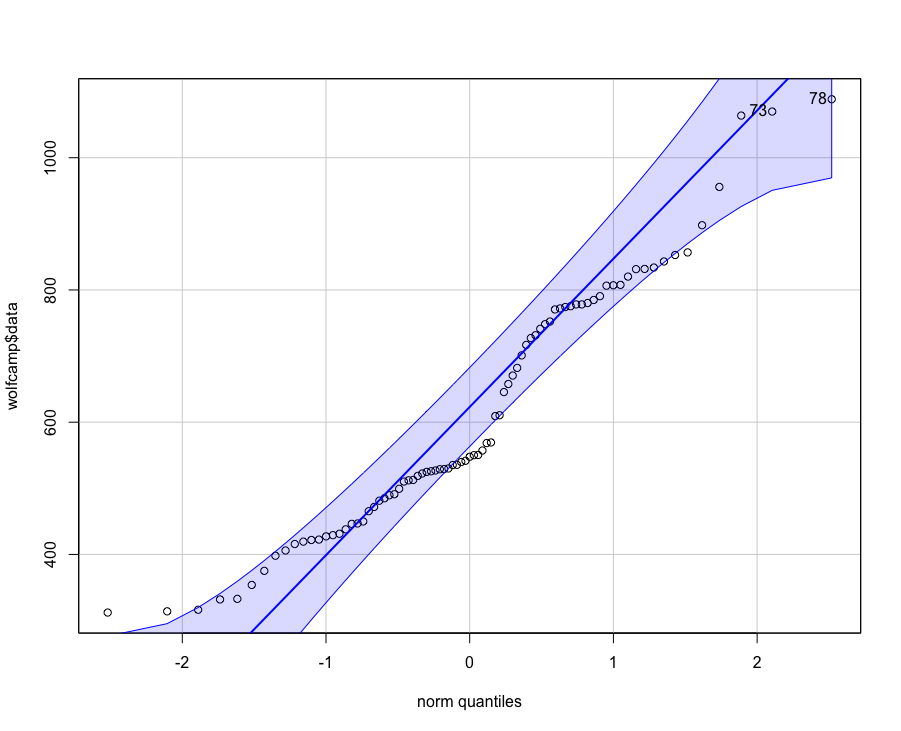
\includegraphics[width = .75\textwidth]{original.png}
    \end{center}
  \end{figure}
  \begin{figure}[H]
    \begin{center}
      \caption{QQ normPlot of root transformed Wolfcamp data.}
    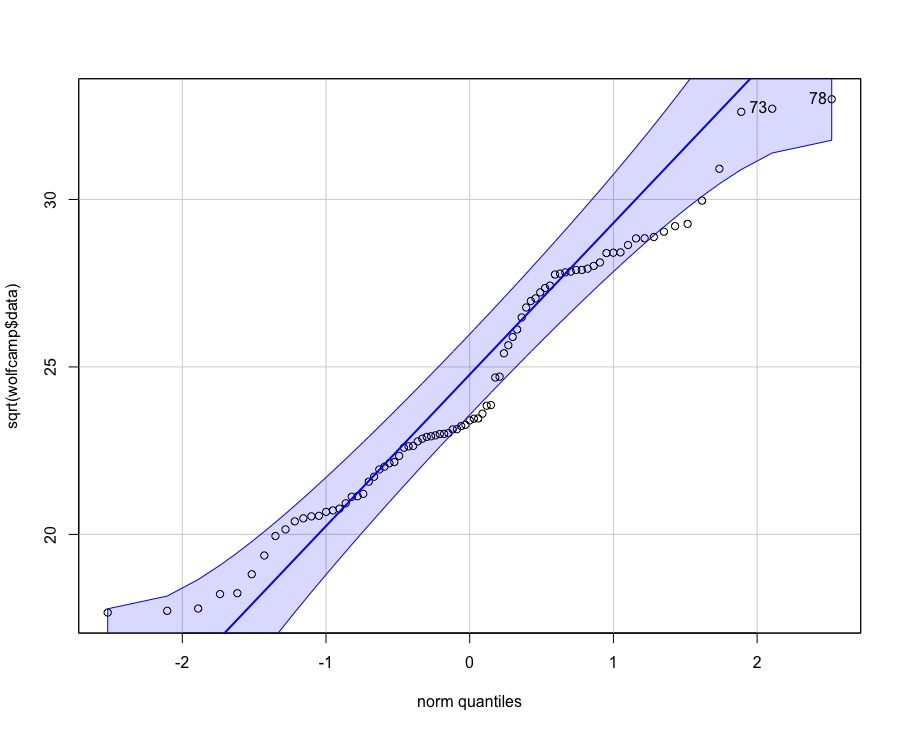
\includegraphics[width = .75\textwidth]{root.png}
    \end{center}
  \end{figure}
  \begin{figure}[H]
    \begin{center}
      \caption{QQ normPlot of log transformed Wolfcamp data..}
    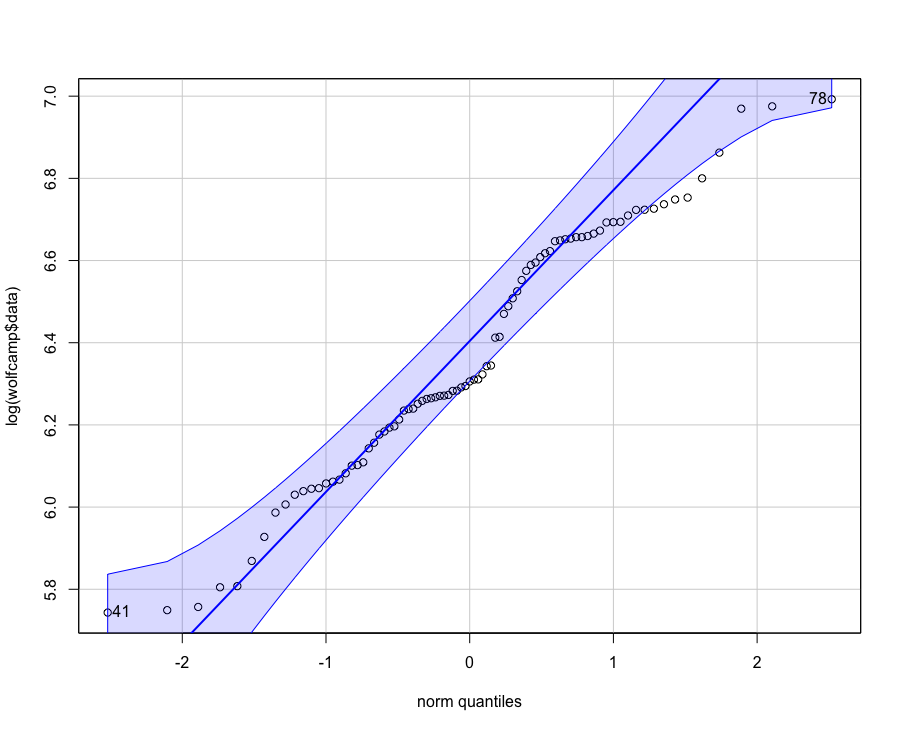
\includegraphics[width = .75\textwidth]{log.png}
    \end{center}
  \end{figure}

  To determine if any trend term might be appropriate, a partial F test using the anova() function states that the second order model 
  explains a significant amount of the variance. Looking at the summary report we can see which terms contain that significance, and we find 
  that the interaction and second order latitude are the most significant of the second order terms. Moving forward we will consider the second order trend. (Although it's not included 
  I found that centered locations produced almost identical models.) \\
  \textbf{Code:}
  \begin{center}
  \lstinputlisting[basicstyle = \footnotesize]{r4.txt}
  \end{center}
  



  Given that we know will consider variograms with second order trend we can now construct an empirical semivariogram. We will be using the robust empirical semivariogram estimator, but before we move on 
  to estimating the semivariogram we must consider a few diagnostic concerns. Do we even need a spatial model? Does the data exhibit anisotropy? We will address the need for constructing a spatial model first. 
  Testing for spatial autocorrelation using a randomization test we can see that the empirical semivariogram for our original data shows a clear trend amongst the randomized empirical semivariograms, we need 
  a spatial model. 
  
  \begin{figure}[H]
    \begin{center}
      \caption{Randomization test for spatial autocorrelation. (red is the original data)}
    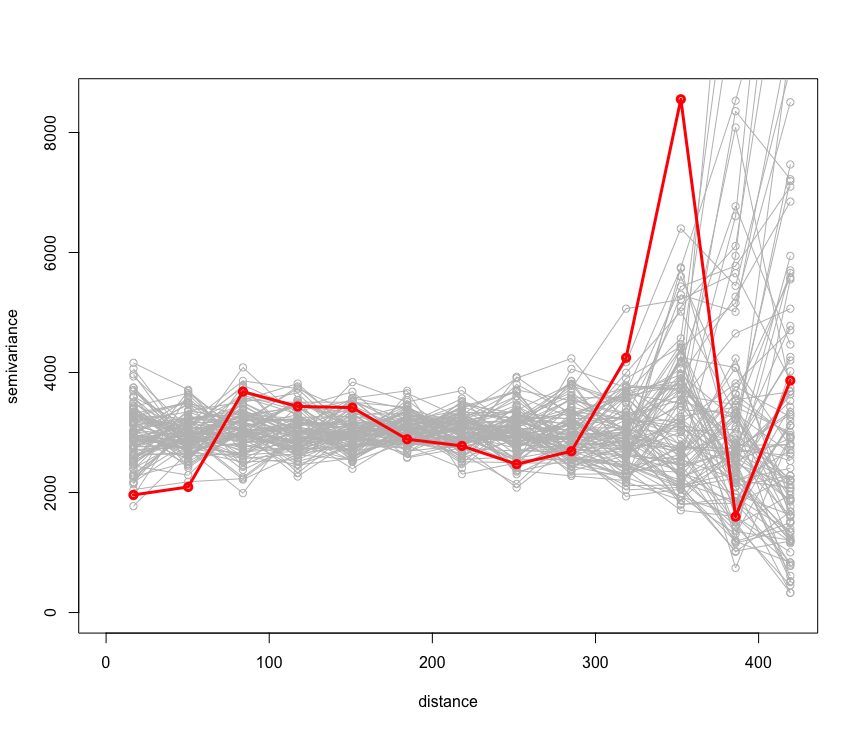
\includegraphics[width = .75\textwidth]{Rplot02.png}
    \end{center}
  \end{figure}
  \textbf{Code:}
  \begin{center}
  \lstinputlisting[basicstyle = \footnotesize]{r5.txt}
  \end{center}
  To check for anisotropy we will construct 4 directional empirical semivariograms using the variog4() function in geoR. Doing so we find that the variance in each direction 
  seems to stay the same, except for lags in the range of 300 to 350. This makes sense then we look at the spatial trend and distribution in our data, however what is most important is 
  where we have data in the lower range from 0 to 250 we see very similar variances. 

  \begin{figure}[H]
    \begin{center}
      \caption{Testing for anisotropy with directional semivariograms}
    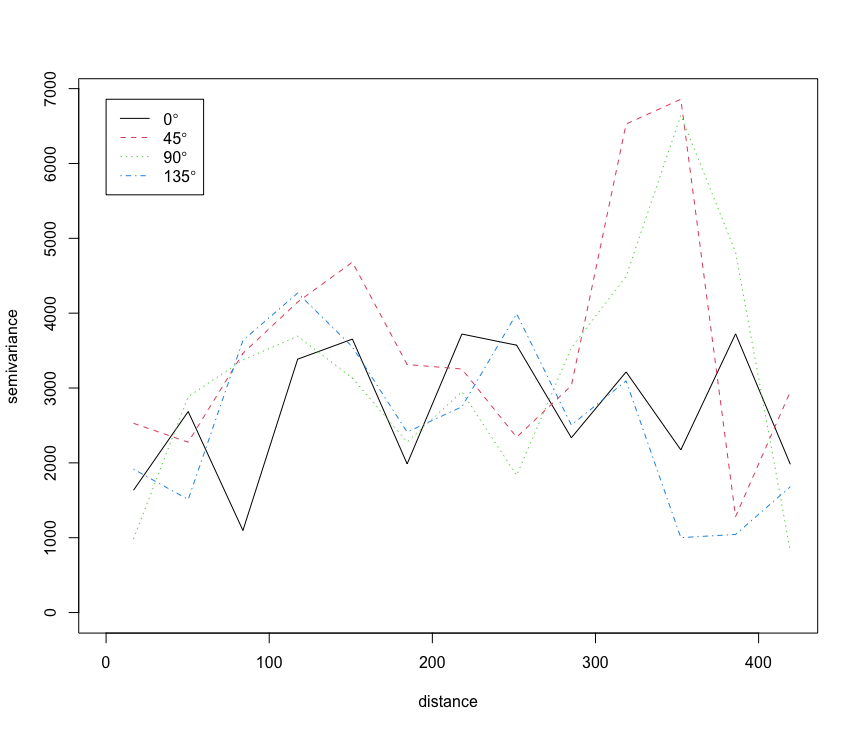
\includegraphics[width = .75\textwidth]{Rplot03.png}
    \end{center}
  \end{figure}
  \textbf{Code:}
  \begin{center}
  \lstinputlisting[basicstyle = \footnotesize]{r6.txt}
  \end{center}

  Having roughly tested the assumptions of isotropic second order stationarity we can continue by considering what type and technique we are going to use 
  to estimate the variogram. Using eyefit() to find initial values for each type of semivariogram we get the following, 
  
  \begin{figure}[H]
    \centering
    \caption{Eyefit() plots.}
    \begin{subfigure}[b]{0.45\textwidth}
        \centering
        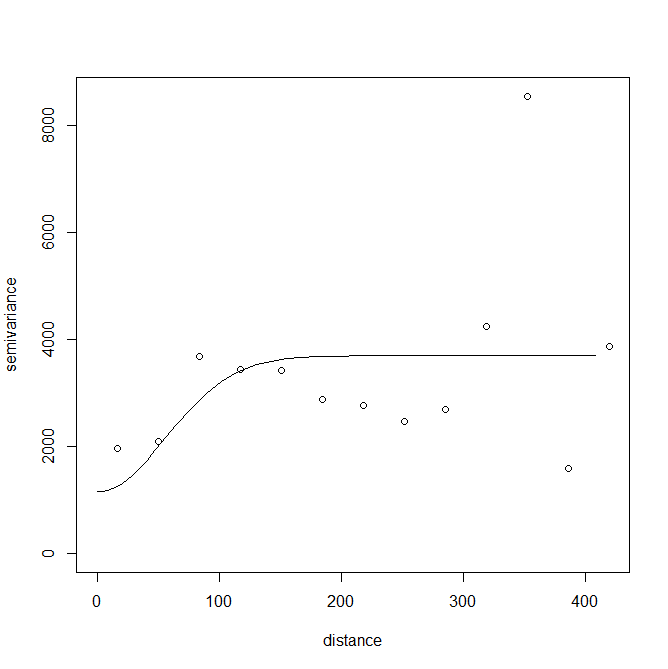
\includegraphics[width=\textwidth]{Gaussian.png}
        \caption{Gaussian}
    \end{subfigure}
    \hfill
    \begin{subfigure}[b]{0.45\textwidth}
        \centering
        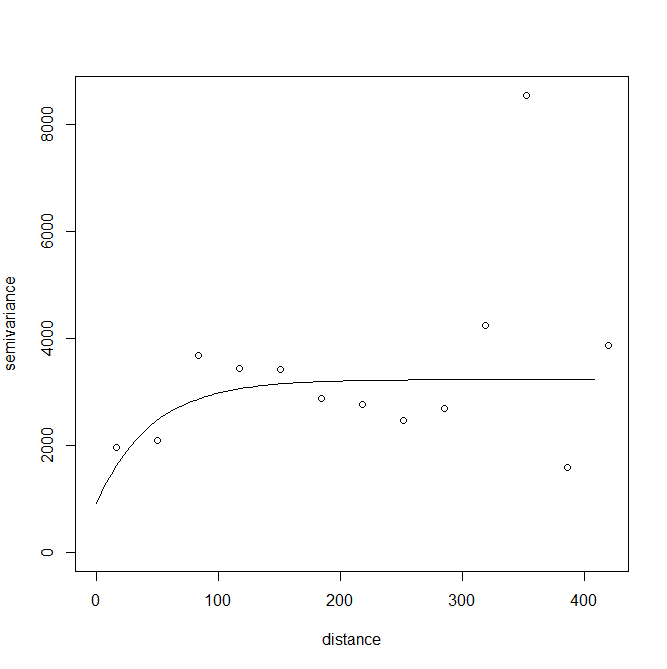
\includegraphics[width=\textwidth]{Exponential.png}
        \caption{Exponential}
    \end{subfigure}
    \hfill
    \begin{subfigure}[b]{0.45\textwidth}
        \centering
        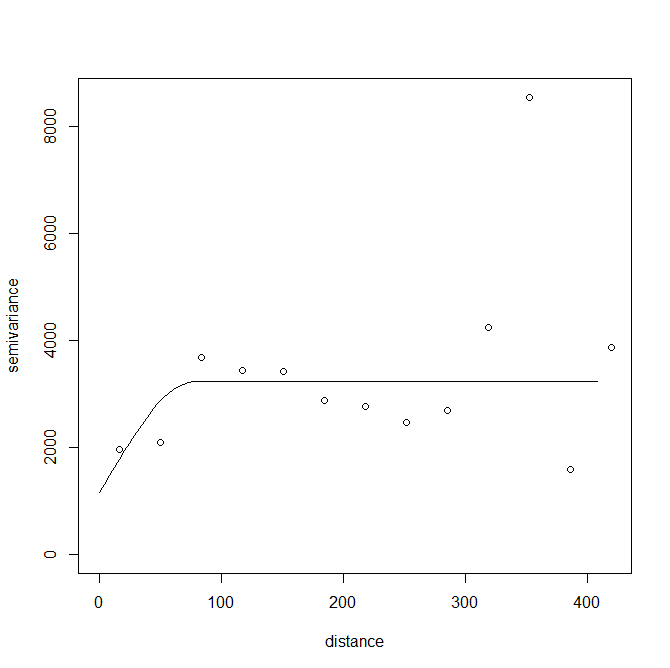
\includegraphics[width=\textwidth]{Spherical.png}
        \caption{Spherical}
    \end{subfigure}
\end{figure}

\begin{figure}[H]
  \begin{center}
    \caption{Initial values from eyefit()}
  \begin{tabular}{|c||c|c|c| }
    \hline
     & $\sigma^2$ & $\phi$ & $\tau^2$\\
    \hline 
    \hline
    Gaussian    & 2543 & 79.35 & 1155.91 \\   
    Exponential & 2311 & 45.34 & 924.73\\ 
    Spherical   & 2080 & 79.35 &  1155.91\\ 
    \hline
   \end{tabular}
  \end{center}
\end{figure}

Using these initial values we can fit the WLS estimator, 
then subsequently the ML and REML estimators. Doing so we get the following.

\begin{figure}[H]
  \begin{center}
    \caption{WLS estimated semivariograms.}
  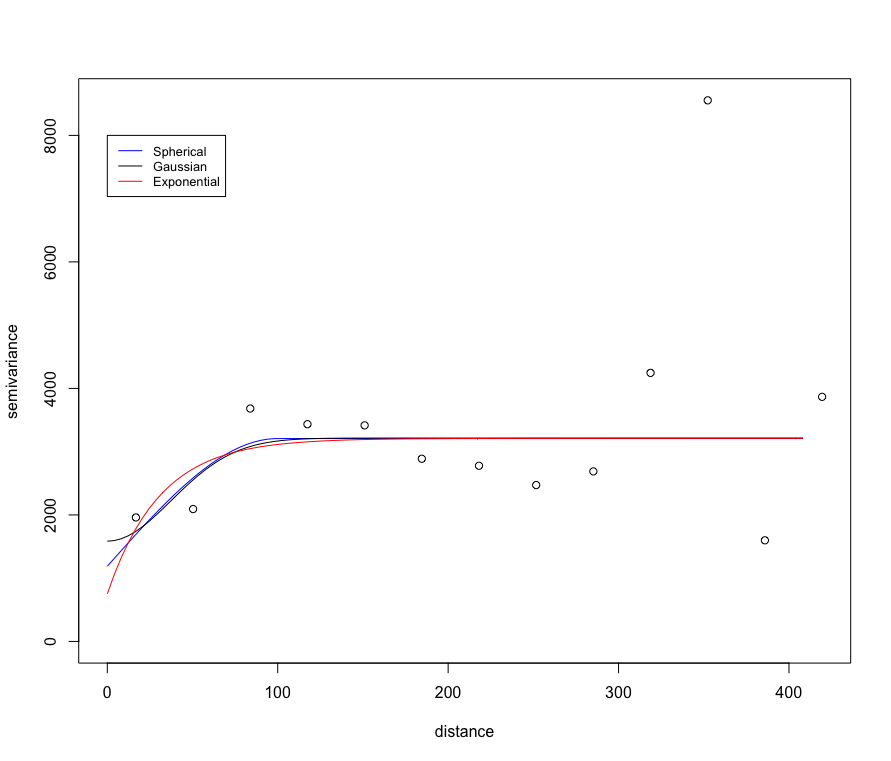
\includegraphics[width = \textwidth]{Rplot04.png}
  \end{center}
\end{figure}
\begin{figure}[H]
  \begin{center}
    \caption{ML estimated semivariograms.}
  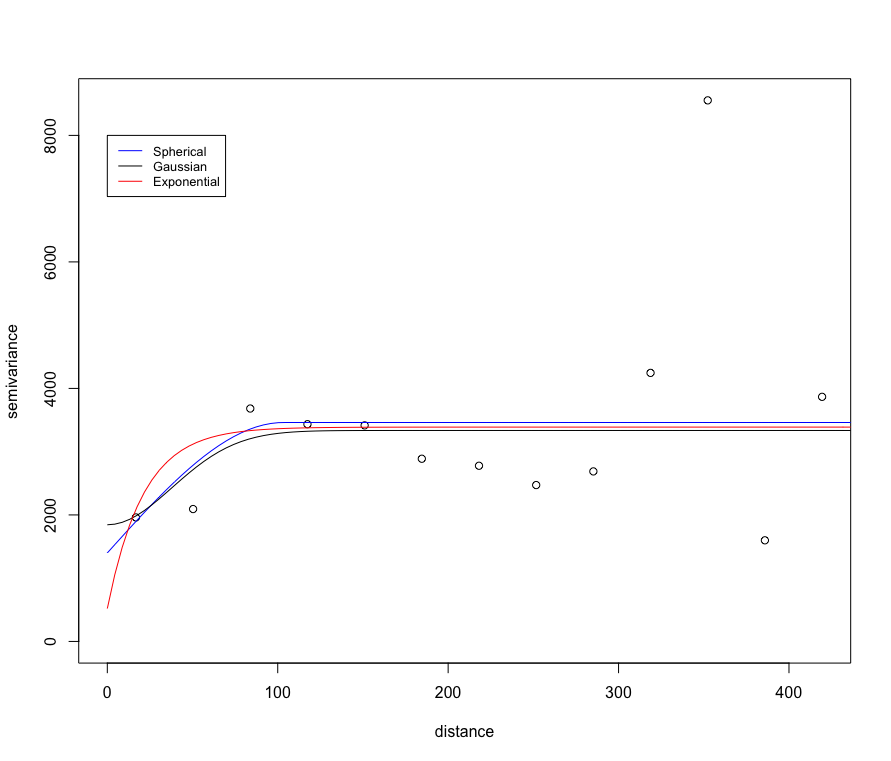
\includegraphics[width = \textwidth]{Rplot05.png}
  \end{center}
\end{figure}
\begin{figure}[H]
  \begin{center}
    \caption{REML estimated semivariograms.}
  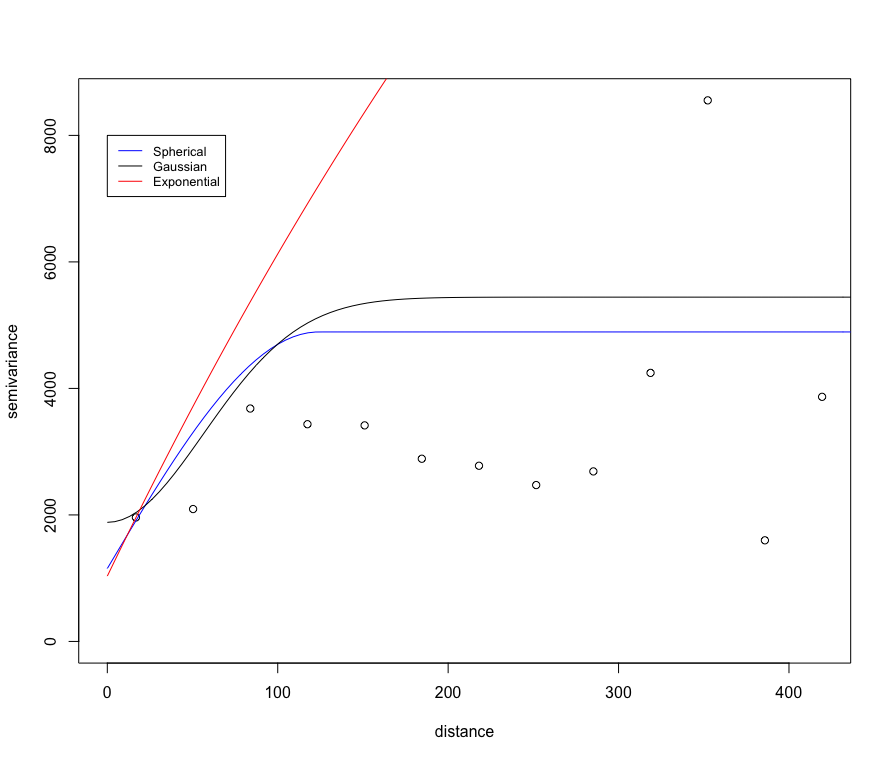
\includegraphics[width = \textwidth]{Rplot06.png}
  \end{center}
\end{figure}

\textbf{Code:}
\begin{center}
\lstinputlisting[basicstyle = \footnotesize]{r7.txt}
\end{center}


Generally it seems as though the REML estimator does a poor job at estimating the semivariogram. Beyond that it 
seems that the WLS and ML estimators generally do a good job at estimating the semivariogram. We can see that there is 
larger variance among the ML estimated variograms. Computing the AIC for each ML estimator we get the following table, 


\begin{figure}[H]
  \begin{center}
    \caption{Computed AIC values from ML estimated models.}
  \begin{tabular}{|c||c|}
    \hline
                 & AIC \\
    \hline 
    \hline
    Gaussian    & 929.7375 \\
    Exponential & 927.8655 \\
    Spherical   & 928.1551 \\
    \hline
   \end{tabular}
  \end{center}
\end{figure}

Here we see that exponential model exhibits the best fit. Comparing the WLS and ML exponential models we see that, the ML model seems to 
have a larger sill favoring the larger lags in the 300 to 400 region. Moving forward we will be considering the ML exponential model. 

\begin{figure}[H]
  \begin{center}
    \caption{ML vs WLS exponential semivariograms.}
  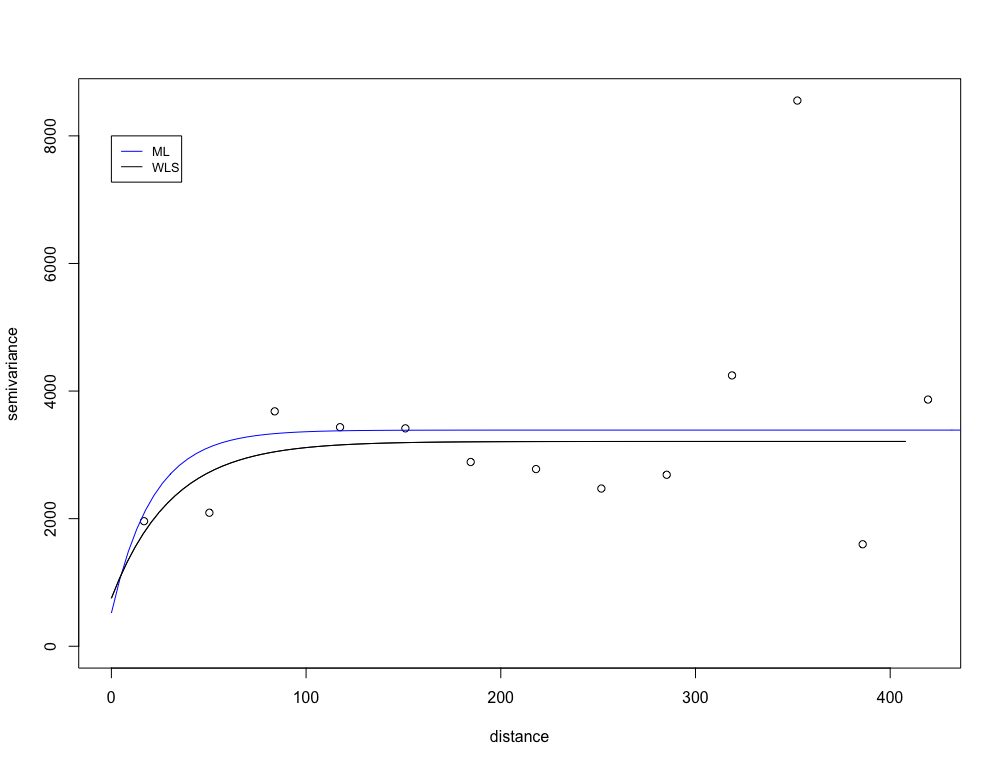
\includegraphics[width = \textwidth]{Rplot07.png}
  \end{center}
\end{figure}

\textbf{Code:}
\begin{center}
\lstinputlisting[basicstyle = \footnotesize]{r8.txt}
\end{center}

Since we are including a second order trend we will continue by using universal kriging to create a smoothed map of 
the wolfcamp data. Using the krig.control() and krig.conv() functions we get the following, 

\begin{figure}[H]
  \begin{center}
  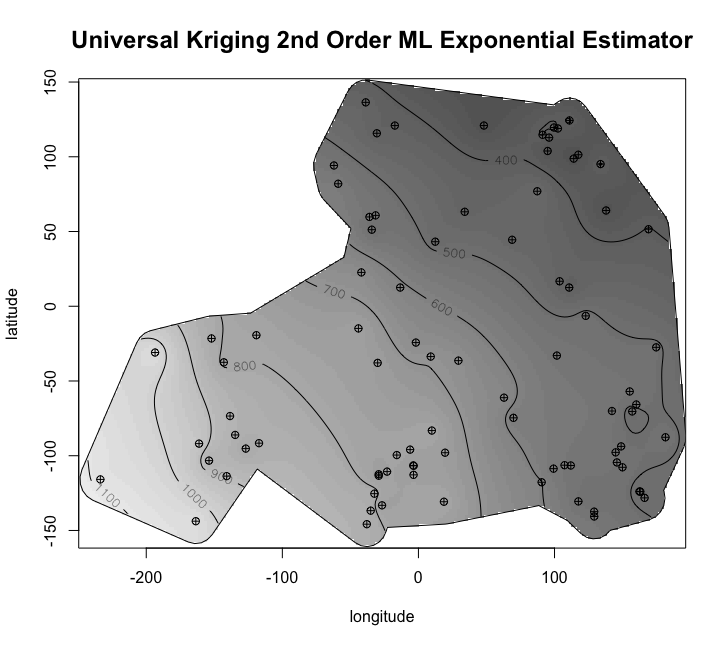
\includegraphics[width = \textwidth]{Rplot08.png}
  \end{center}
\end{figure}
\textbf{Code:}
\begin{center}
\lstinputlisting[basicstyle = \footnotesize]{r9.txt}
\end{center}
Calling my\_kr\_results\$beta.est we get the final estimated regression equation, 
\begin{equation*}
  \mathbb{E}(Y(s)) =  617.3-1.2lon -1.3lat + .00098lon^2 -.0027lat^2+ .0024lonlat.
\end{equation*}
This final fitted model is kind of similar to our non spatial second order model, 
\begin{equation*}
  \mathbb{E}(Y(s)) =  620.3-1.0lon -1.3lat + .00089lon^2 -.0029lat^2+ .0032lonlat.
\end{equation*}
They both exhibit the same significance in the $lat^2$ and interaction terms. 
\end{exercise}
\vspace{1in}





\begin{exercise}{3} Fit a Bayesian model to these data by modifying the R code, Bayesian\_kriging.r, which is posted on Canvas. 
  Be sure to include diagnostic plots shown in class (traceplots and density plots for the model parameters) and a final smoothed map.\\
  \solution Using the Bayesian\_kriging.r R code to fit a Bayesian model, we get the following smoothed map(A lower resolution was used to save computational time),  
  \begin{figure}[H]
    \begin{center}
    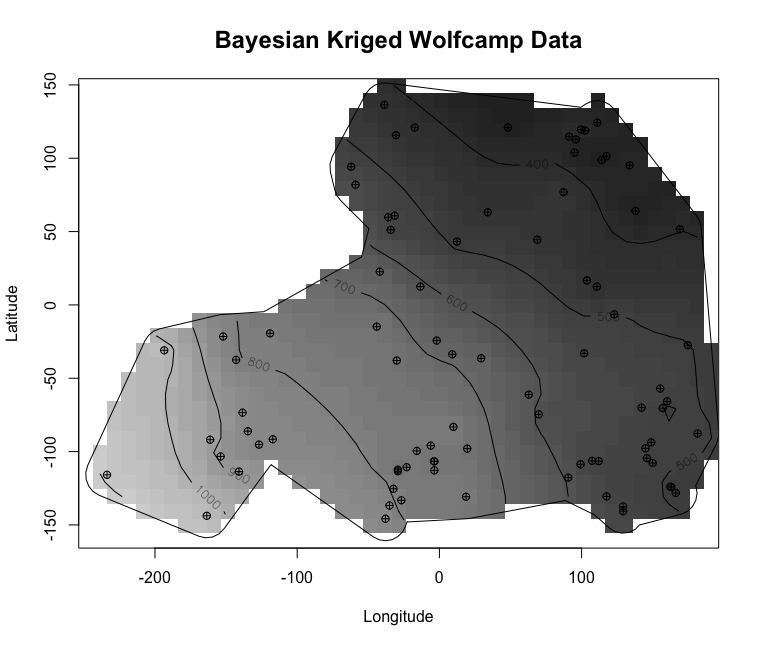
\includegraphics[width = \textwidth]{Rplot09.png}
    \end{center}
  \end{figure}
  The Bayesian model produced the following 95\% credible set, smoothed maps
  \begin{figure}[H]
    \begin{center}
    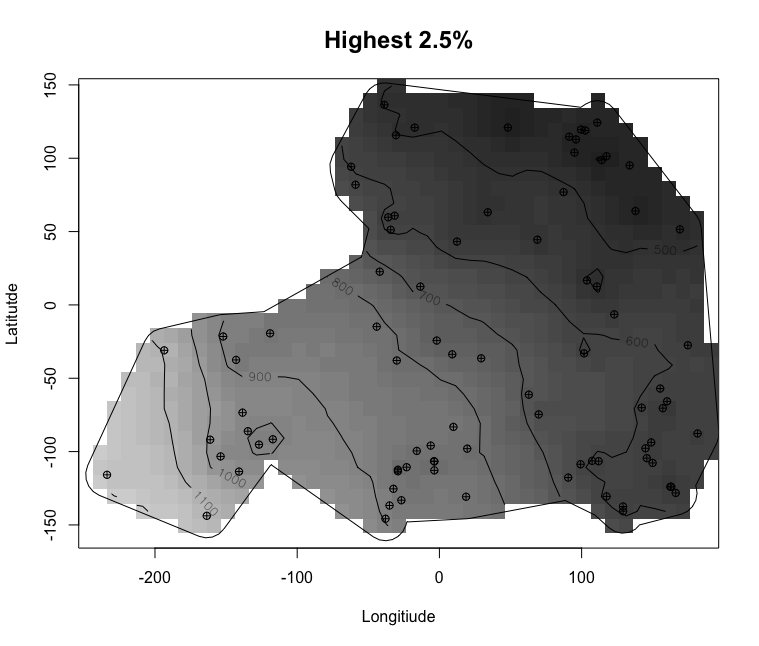
\includegraphics[width = \textwidth]{Rplot10.png}
    \end{center}
  \end{figure}
  \begin{figure}[H]
    \begin{center}
    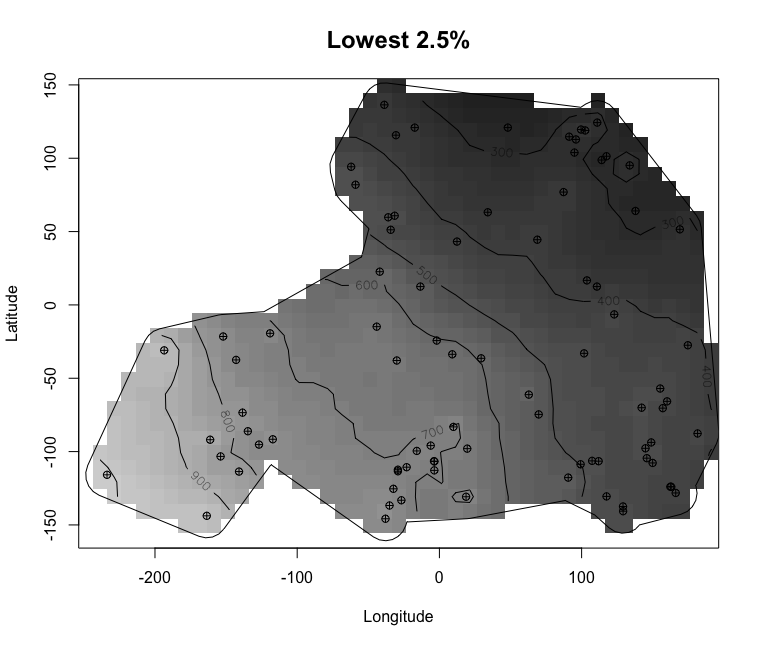
\includegraphics[width = \textwidth]{Rplot11.png}
    \end{center}
  \end{figure}

  The Bayesian model also produced the following trace plots for each parameter from the 5000 posterior distribution samples (Draws were plotted at interval of 
  every 10 draws, hence 500 iterations). Looking at traceplots for the $\beta_i$ parameters, show relatively good convergence. Of the 6 parameters, it seems as though 
  $\beta_0$ has the highest variance, yet the density looks very normal this is likely do to the fact that our location data are not centered or scaled(the plot looks to have more variance and poor convergence). 
  We also see $\beta_1$ exhibit some level of burn-in, around iteration 250 we see the the parameter level off. The $\sigma^2$ trace plot looks normal given that it is a non-negative parameter. The variance exhibited in the 
  $\phi$ trace plot tells us that our data is not saying much about the value of the range. This conclusion makes sense given the shape of our empirical semivariogram, it seems as though since it is very flat, in large part, what is going to determine 
  the shape of the estimated semivariogram is the sill and the nugget and range parameters from 0 to 100 will still fit fairly well. 
  \begin{figure}[H]
    \begin{center}
    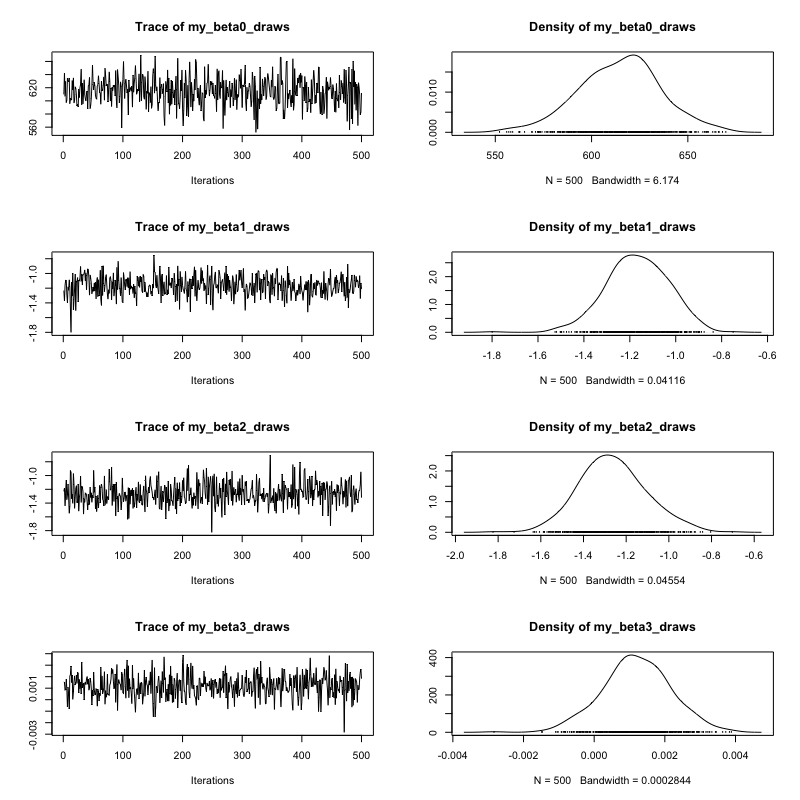
\includegraphics[width = \textwidth]{Rplot14.png}
    \end{center}
  \end{figure}
  \begin{figure}[H]
    \begin{center}
    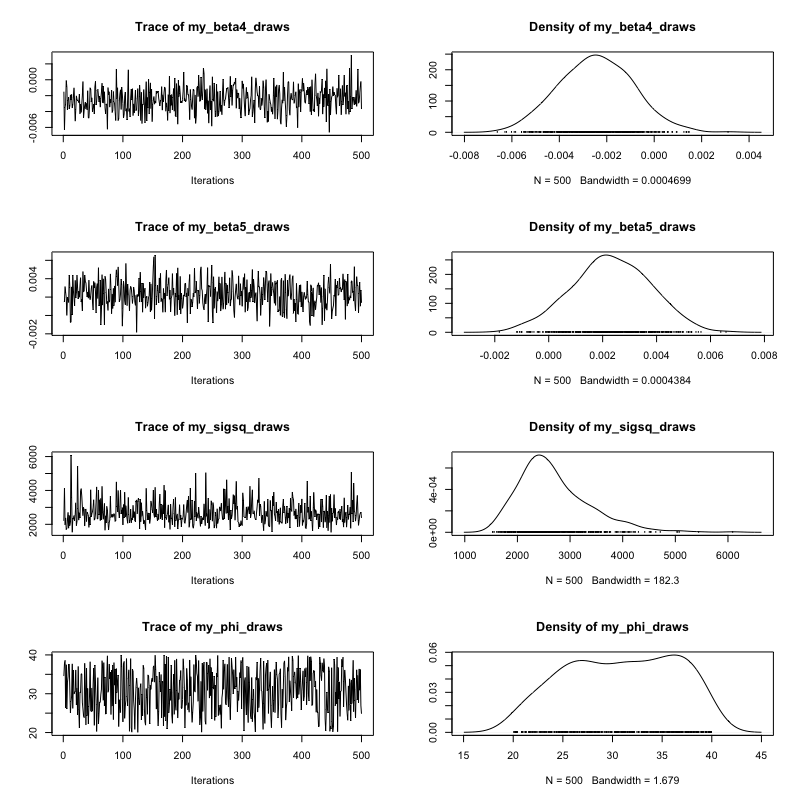
\includegraphics[width = \textwidth]{Rplot15.png}
    \end{center}
  \end{figure}
  \begin{figure}[H]
    \begin{center}
    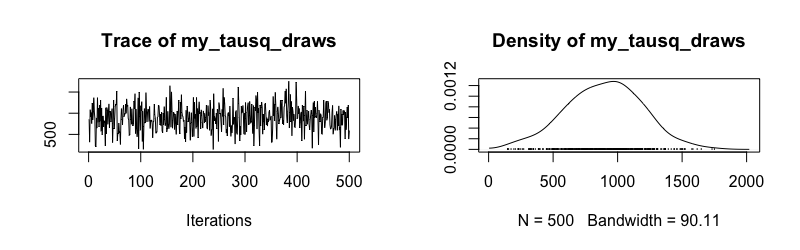
\includegraphics[width = \textwidth]{Rplot16.png}
    \end{center}
  \end{figure}
  \textbf{Code:}
  \begin{center}
  \lstinputlisting[basicstyle = \footnotesize]{r10.txt}
  \end{center}
  

  Considering the correlation between our semivariogram parameters we get the following plots. 
  \begin{figure}[H]
    \centering
    \caption{Scatterplots for Semivariogram parameters.}
    \begin{subfigure}[b]{0.45\textwidth}
        \centering
        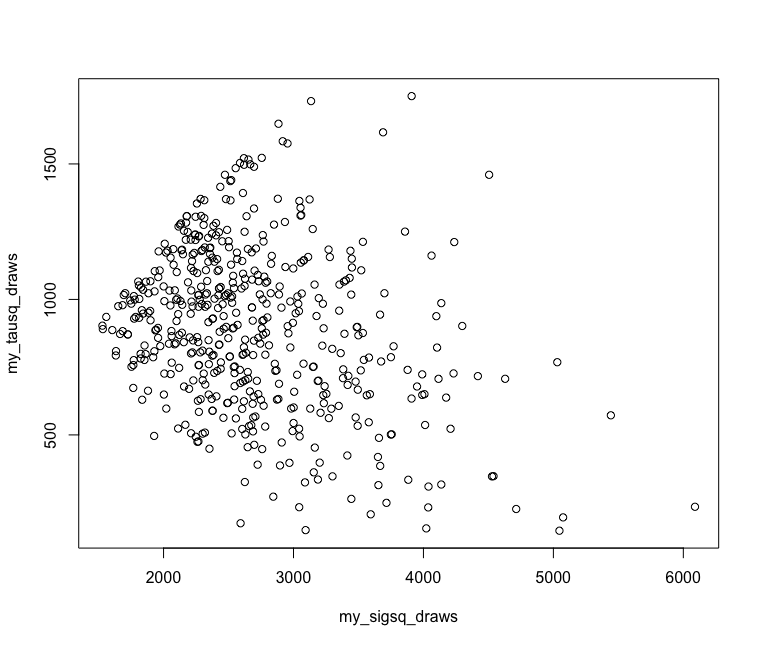
\includegraphics[width=\textwidth]{Rplot17.png}
        \caption{$\sigma^2$ vs $\tau^2$}
    \end{subfigure}
    \hfill
    \begin{subfigure}[b]{0.45\textwidth}
        \centering
        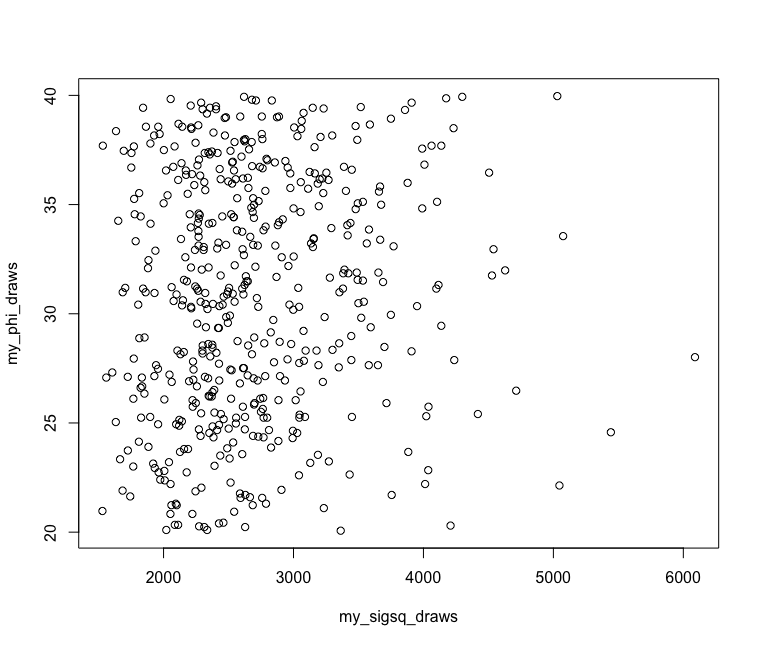
\includegraphics[width=\textwidth]{Rplot18.png}
        \caption{$\sigma^2$ vs $\phi$}
    \end{subfigure}
    \hfill
    \begin{subfigure}[b]{0.45\textwidth}
        \centering
        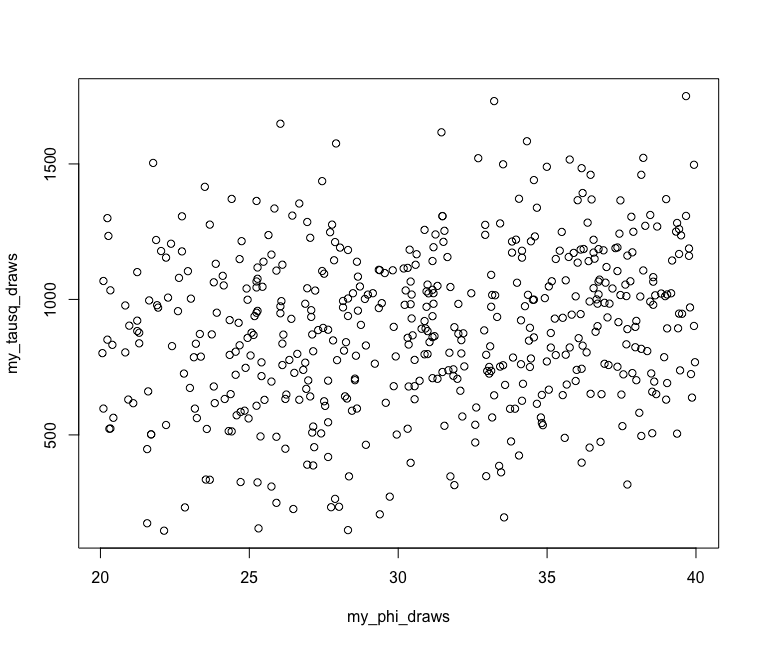
\includegraphics[width=\textwidth]{Rplot19.png}
        \caption{$\phi$ vs $\tau^2$}
    \end{subfigure}
\end{figure}
  As we can see the plots show relatively little correlation, with the most significant 
  computed correlation being -.29 between $\sigma^2$ and $\tau^2$. \\
  \textbf{Code:}
  \begin{center}
  \lstinputlisting[basicstyle = \footnotesize]{r11.txt}
  \end{center}
\end{exercise}
\vspace{1in}



\begin{exercise}{4} State the statistical model you are using. This means: state the likelihood and state the prior 
  distribution for the various parameters in the model. Page 118 of the lecture notes shows an example of what I mean by this. Also, be sure 
  to state the posterior distribution, for example, as show on page 119 of the class notes.\\ 
  \solution Stating our likelihood and priors similarly to page 118 we get the following. Note that $\hat{\beta} = [\beta_0, ... \beta_5]$, n is the number of 
  observations in the wolfcamp datam $X$ is our second order design matrix, and $\Sigma$ is our covariance matrix (I think we should be replacing it with $S^2$).  
  \begin{align*}
    Y &\sim MVN_n\left(X\hat{\beta}, \Sigma \right)\\
    \hat{\beta} &\sim MVN_6 \left([600, 0, 0, 0, 0, 0],10000I_6 \right)\\
    \sigma^2 &\sim 1/\sigma^2 (\sigma^2 > 0)\\ 
    \phi &\sim uniform[20 \dots 60]\\
    \omega &\sim  uniform[0.01 \dots 0.6]
  \end{align*}
  Stating the posterior distribution we get the following. Let $\theta = (\hat{\beta}, \sigma^2, \phi, \omega)$.
  \begin{align*}
    p(\theta | y) &\propto L(\theta)\pi(\hat{\beta})\pi(\sigma^2)\pi(\phi)\pi(\omega)\\ 
    &\propto \dfrac{1}{\sqrt{(2\pi)^n}\det(\Sigma)} \exp(-\dfrac{1}{2}(y - X\hat{\beta})^T\Sigma^{-1}(y - X\hat{\beta}))\\ 
    &\times \dfrac{1}{\sqrt{2\pi(10^4)}} \exp\left(-\dfrac{1}{2(10^4)}(\beta_0 - 600)^2\right) \times \prod_{i = 1}^5 \dfrac{1}{\sqrt{2\pi(10^4)}} \exp\left(-\dfrac{1}{2(10^4)}\beta_i^2\right)\\
    &\times \dfrac{1}{\sigma^2} (\sigma^2 > 0)\\
    &\times I(\phi \in [20 \dots 60])\\
    &\times I(\omega \in [0.01 \dots .6])
  \end{align*}
\end{exercise}
\vspace{1in}




\begin{exercise}{5} Summarize the (marginal) posterior distributions of the model parameters in a table; one row for each paramater and 
  the following columns for each:
  \begin{enumerate}
    \item posterior mean
    \item posterior standard deviation
    \item posterior median
    \item 95\% credible set 
    \item Monte Carlo error
    \item Effective sample size.
  \end{enumerate}
  \solution By calling summary on the mcmc(my\_bayes\_results\$posterior\$sample) we get a fairly thorough summary report. Note that this command 
  is creating an mcmc object on all 5000 samples from the posterior distribution therefore it includes no thinning, and any burn-in samples. From our trace 
  plots we saw that really only $\beta_1$ exhibited any burn in, so for the following table we used the 'start = '  paramater to remove those samples. 
  \begin{figure}[H]
    \begin{center}
      \caption{Marginal Posterior Distributions Summary}
    \begin{tabular}{|c||c|c|c|c|c|c| }
      \hline
       &  $\mu$ & $\sigma$ & median & 95\% CS & MC err. & Effec.samp.size\\
      \hline 
      $\beta_0$  & 614.4      &  22.10      & 614.6     & (570.3, 658.2)     & .3125     & 5000 \\
      $\beta_1$  &-1.16       &  .133       &-1.16      & (-1.42, -.896)     & .00188    & 5000 \\
      $\beta_2$  &-1.27       &  .157       &-1.267     & (-1.57, -.940)     & .00222    & 5000 \\
      $\beta_3$  & .00119     &  .000965    & .00116    & (-.00068, .000317) & .0000136  & 5000 \\
      $\beta_4$  &-.00248     &  .00164     &-.00249    & (-.00567, .000754) & .0000232  & 5000 \\
      $\beta_5$  & .00230     &  .00148     & .002308   & (-.000598, .00523) & .0000209  & 4883 \\
      $\sigma^2$ & 2687       &  690.3      & 2559      & (1728, 4410)       & 9.76      & 5000 \\
      $\phi$     & 31.1       &  5.490      & 31.45     & (20.90, 39.63)     & .0776     & 5000 \\
      $\omega$   & .362       &  .149       & .372      & (.0764, .591)      & .00211    & 5000 \\
      \hline
      \hline
     \end{tabular}
    \end{center}
  \end{figure}
  \textbf{Code:}
  \begin{center}
  \lstinputlisting[basicstyle = \footnotesize]{r12.txt}
  \end{center}
\end{exercise}
\vspace{1in}




\begin{exercise}{6} Provide a summary of your results; specifically, 
  \begin{enumerate}
    \item How many iterations did you use for your MCMC, and how much thinning (if any) did you do? What about burn-in?\\
    \solution Our MCMC algorithm utilized 5000 iterations to sample the posterior distribution and 1000 iterations of kriged surfaces sampled 
    from the predictive posterior distribution. We used some thinning to visualize the trace plots as pointed out previously, and we also experience some 
    burn-in on the $\beta_1$ parameter. When computing the summary report for the marginal posterior distributions we did not use any thinning, and 
    we computed the values for the $\beta_1$ distribution excluding the burn-in samples (although it didn't change really). 



    \item Discuss the convergence of the MCMC for the Bayesian model. Do the various plots indicate any issues with convergence?
    What do the Monte Carlo errors suggest about convergence or lack of convergence?\\
    \solution Generally the trace plots do not exhibit any issues with convergence. Notably the traceplot for the $\phi$ parameter seems to exhibit a wide range 
    of values, which is more indicative of behavior/quality of our data rather than any non-convergence that might appear from an ill-calibrated priori. The $\beta_1$ traceplot
    showes signs of burn-in however quickly levels off, indicateing good convergence.  Using the crude 10\% 
    test that we discussed during lecture, we find that $\beta_3$ could likely be ran a little longer since, $.0000119 < .0000136$, however the difference seems really small and 
    the trace plot really shows no sign of poor convergence. 
  \end{enumerate}
\end{exercise}
\vspace{1in}



\begin{exercise}{7} Discuss (briefly) whether your results for the frequentist and Bayesian approaches are similar; are there any major differences? 
  (A table plus discussion is the best way to do this.)\\
  \solution Considering the model parameters for both approaches, 
  \begin{figure}[H]
    \begin{center}
      \caption{Model Parameters Frequentist vs Bayesian}
    \begin{tabular}{|c||c|c|c|c|c|c|c|c|c| }
      \hline
       &$\beta_0$ & $\beta_1$ & $\beta_2$ & $\beta_3$ & $\beta_4$ & $\beta_5$ & $\sigma^2$& $\phi$    & $\tau^2$ \\ 
      \hline 
      Frequentist &  617.1    & -1.15     & -1.31     &  .0010    & -.0027    &  .0024    & 2458       & 30.9   & 752.123\\
      Bayesian    & 614.4     &-1.16      &-1.27      & .0012     &-.0025     & .0023     & 2687      & 31.1   & 899.415\\
      \hline
     \end{tabular}
    \end{center} 
  \end{figure}
  We see the biggest differences in the variogram parameters of our model. Its clear that the Bayesian model has a significantly higher 
  nugget and larger range. Graphing the two semivariograms we get the following, 
  \begin{figure}[H]
    \begin{center}
    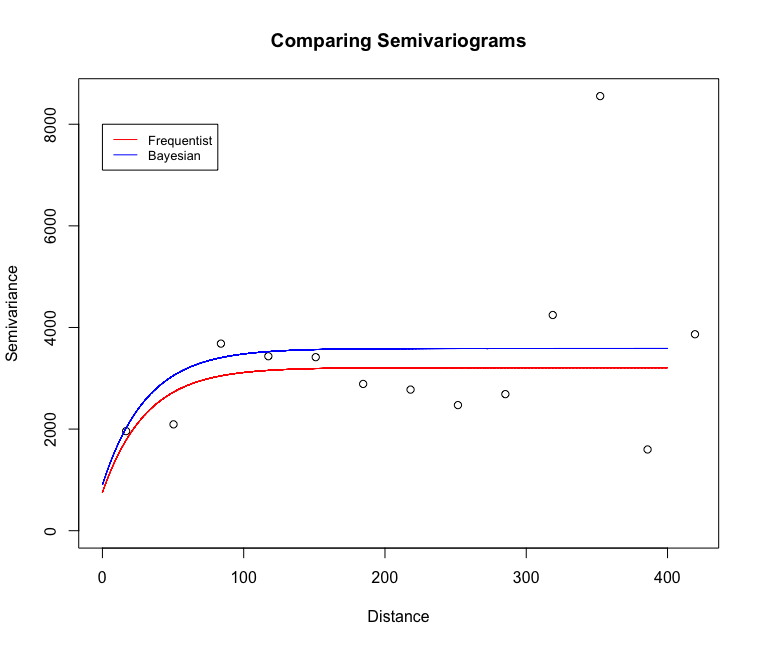
\includegraphics[width = \textwidth]{Rplot20.png}
    \end{center}
  \end{figure}
  \textbf{Code:}
  \begin{center}
  \lstinputlisting[basicstyle = \footnotesize]{r13.txt}
  \end{center}
  It seems like the Bayesian model puts a larger emphasis on the larger greater lags, opting for a larger nugget and larger range. This should result in 
  smoother realizations outside of our sample areas, as discussed the problem 1 of the previous homework(comparing the matern semivariograms). To me the results are 
  not significancy better from the bayesian method, to warrant such significant increase in computation time. The drawback of having to limit the resolution of the smoothed map is 
  frustrating, when the model, at least to me does not appear to be significantly better. 



\end{exercise}











\end{document}


















